\documentclass[aps,showpacs,twocolumn,floats,prd,superscriptaddress,nofootinbib]{revtex4} 

\usepackage{amsmath}
\usepackage{latexsym}
\usepackage{graphicx}
\usepackage{epsfig}
\usepackage{verbatim}
\usepackage{hyperref}
\usepackage{url}
\usepackage{color}

\newcommand{\Msun}{\>{\rm M_{\odot}}}
\newcommand{\beq}{\begin{equation}}
\newcommand{\eeq}{\end{equation}}
\newcommand{\bea}{\begin{align}}
\newcommand{\eea}{\end{align}}
\newcommand{\bseq}{\begin{subequations}}
\newcommand{\eseq}{\end{subequations}}
\newcommand{\stm}[1]{({\color{blue}\bf#1--Sean})}
\newcommand{\isy}[1]{({\color{red}\bf#1--I-Sheng})}
\newcommand{\lam}[1]{({\color{green}\bf#1--Lam})}
\def\leq{\raise 0.4ex\hbox{$<$}\kern -0.8em\lower 0.62ex\hbox{$-$}}
\def\geq{\raise 0.4ex\hbox{$>$}\kern -0.7em\lower 0.62ex\hbox{$-$}}
\def\lsim{\raise 0.4ex\hbox{$<$}\kern -0.8em\lower 0.62ex\hbox{$\sim$}}
\def\gsim{\raise 0.4ex\hbox{$>$}\kern -0.7em\lower 0.62ex\hbox{$\sim$}}
\def\pm{\,\raise 0.4ex\hbox{$+$}\kern -0.8em\lower 0.62ex\hbox{$-$}\,}
\def\fht{f_{\rm HT}}
\def\hht{h_{\rm c, \, \, est.}}

\begin{document}

\title{On the pressure-less fluid approximation for large scale structure}
\author{Greg Bryan}
\email{gbryan@astro.columbia.edu}
\affiliation{Department of Astronomy, Columbia University, New York, NY 10027}
\affiliation{Columbia Astrophysics Laboratory, Columbia University, New York, NY 10027}
\author{Rasmi Elasmar}
\email{re2300@columbia.edu}
\affiliation{Department of Astronomy, Columbia University, New York, NY 10027}
\affiliation{Columbia Astrophysics Laboratory, Columbia University, New York, NY 10027}
\author{Lam Hui}
\email{lhui@astro.columbia.edu}
\affiliation{Center for Theoretical Physics, Department of Physics, Columbia University, New York, NY 10027}
\affiliation{Columbia Astrophysics Laboratory, Columbia University, New York, NY 10027}
\date{\today}

%\keywords{gravitational waves --- relativity --- binary stars}

\begin{abstract}
In perturbative studies of large scale structure, it has been customary to employ the
pressure-less fluid approximation -- not that the fluid is strictly
pressure-free, but that pressure can be neglected on the scales of interest.
This was called into question recently. 
It was argued that the discrepancy between standard perturbation 
theory (SPT) and N-body simulations (at the level of tens of percent or more beyond the nonlinear scale) 
should be interpreted as a failure of the pressure-less approximation.
In this paper, we present a series of hydrodynamic simulations (of dark matter as a fluid)
with progressively lower pressure or sound speed, and 
compare them against N-body simulations from the same initial condiitons.
We find that the power spectra from hydrodynamic and N-body simulations agree well
(at the percent level around $k \sim 0.2$ h/Mpc), as long as the sound speed is below 100 km/s.
There is no sign that introducing sound speed improves the agreement. 
On the contrary, if the sound speed is above 100 km/s, results from
hydrodynamic simulations start to deviate significantly from that of the N-body simulations.
This suggests the failure of SPT to match N-body simulations at and beyond the nonlinear scale
is primarily a failure of perturbation theory itself, and {\it not} the failure of the pressure-less approximation.
Effective field theory arguments no doubt correctly
identify pressure as a physical effect that should be present at some level,
but care should be taken in assessing its importance.
At $k \, \gsim \, 0.2$ h/Mpc, non-perturbative methods such as
hydrodynamic simulations should be used for this purpose.
\end{abstract}

\pacs{
04.30.-w % Gravitational waves: theory
04.30.Db, % gravitational wave generation and sources
95.30.Sf % relativity and gravitation
}

\maketitle

\section{Introduction}

{\bf Lam.} Motivation for carrying out this exercise.
Discussion of effective field theory. Also discussion
of the fact that fluid can never be strictly pressure-free;
it's a degenerate limit.

\section{Hydrodynamic simulations}

To compare the fluid and particle models for structure formation, we
employ the {\it Enzo} code \cite{Enzo2014} in two separate modes:
one which solves the Eulerian fluid equations, and the other which
uses the traditional collisionless N-body equations.  Both include
Newtonian gravity in a standard $\Lambda$CDM model with
matter density $\Omega_m = 0.279$, baryon density $\Omega_b = 0.0463$,
dark energy density $\Omega_\Lambda = 0.721$, Hubble constant
$H = 70$ km/s/Mpc, and a primordial power spectral slope of $n=0.972$
and amplitude $\sigma_8 = 0.821$.  Our fiducial box
size is 200 Mpc/h modeled with either $1024^3$ grids or particles;
we use the MUSIC package \cite{MUSIC} to initialize the box at $z=50$ and evolve
to $z=0$.  

For the fluid equations, we adopt the ZEUS solver in Enzo,
largely because it is fast, robust and easy to modify the equation of state.
We explore the impact of varying these choices in the appendix, finding
that over the ranges presented below, the results are insensitive to our
numerical choices.  We explore two ways to determine the pressure, the 
first (``adiabatic"), assumes




%{\bf Greg.} 
%Discussion of the hydrodynamic code, and the simulations
%we have run. Discussion of the distinction between adiabatic and
%isothermal. Discussion of what happens at shocks



\begin{figure}[htb]
\begin{center}
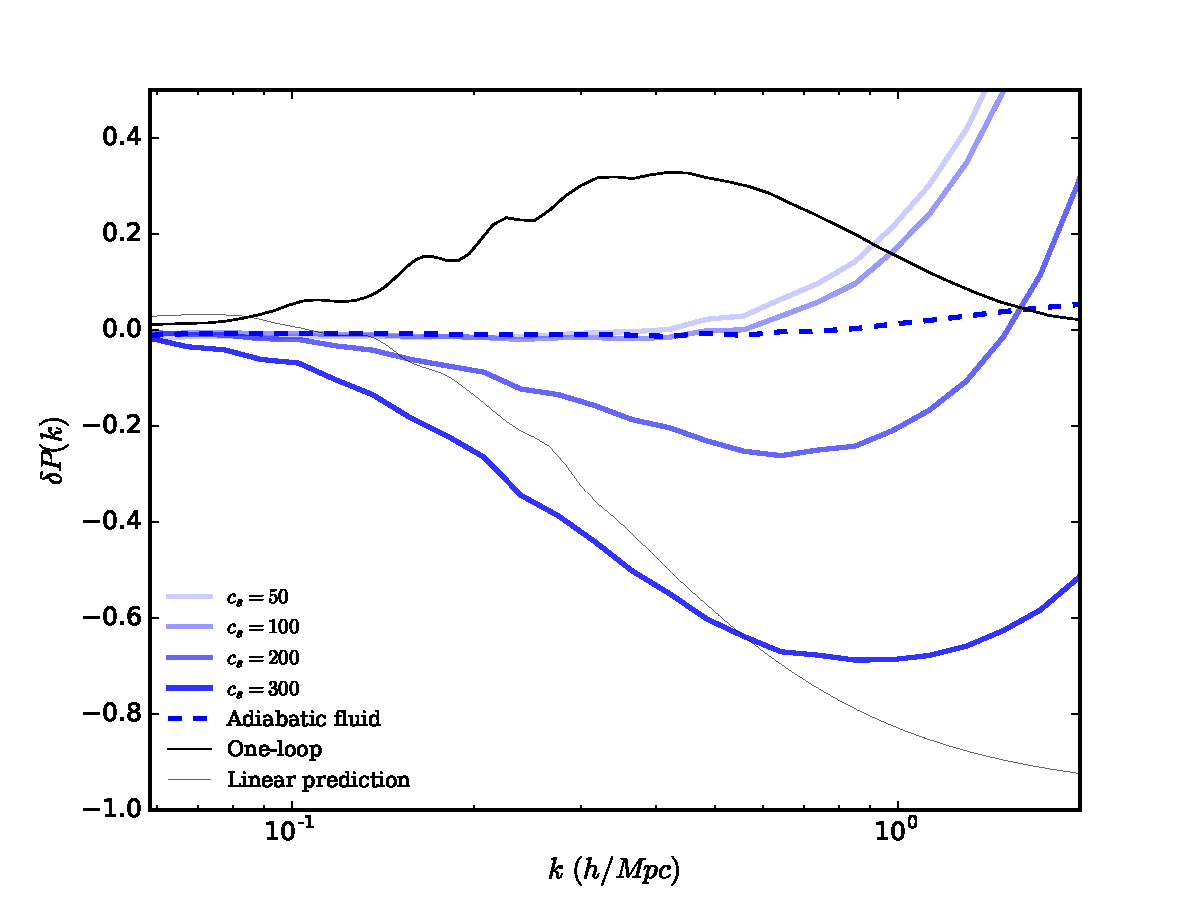
\includegraphics[width=0.48\textwidth]{z0fig}
\end{center}
\caption
{
}
\label{z0fig}
\end{figure}

\section{Discussion}

{\bf Lam.} Conclusion and ideas for future investigation.

\vspace{0.1in}

\section*{Acknowledgements} 
We thank Roman Scoccimarro for useful discussions, and for kindly providing
the one-loop power spectrum.
This work was supported by the DOE and NASA under cooperative agreements
DE-SC0011941 and NNX16AB27G. 

\appendix

\section{Tests}

{\bf Rasmi.} Tests should include: match with linear theory prediction
at $z=10$; box size tests; resolution tests.

\begin{figure}[htb]
\begin{center}
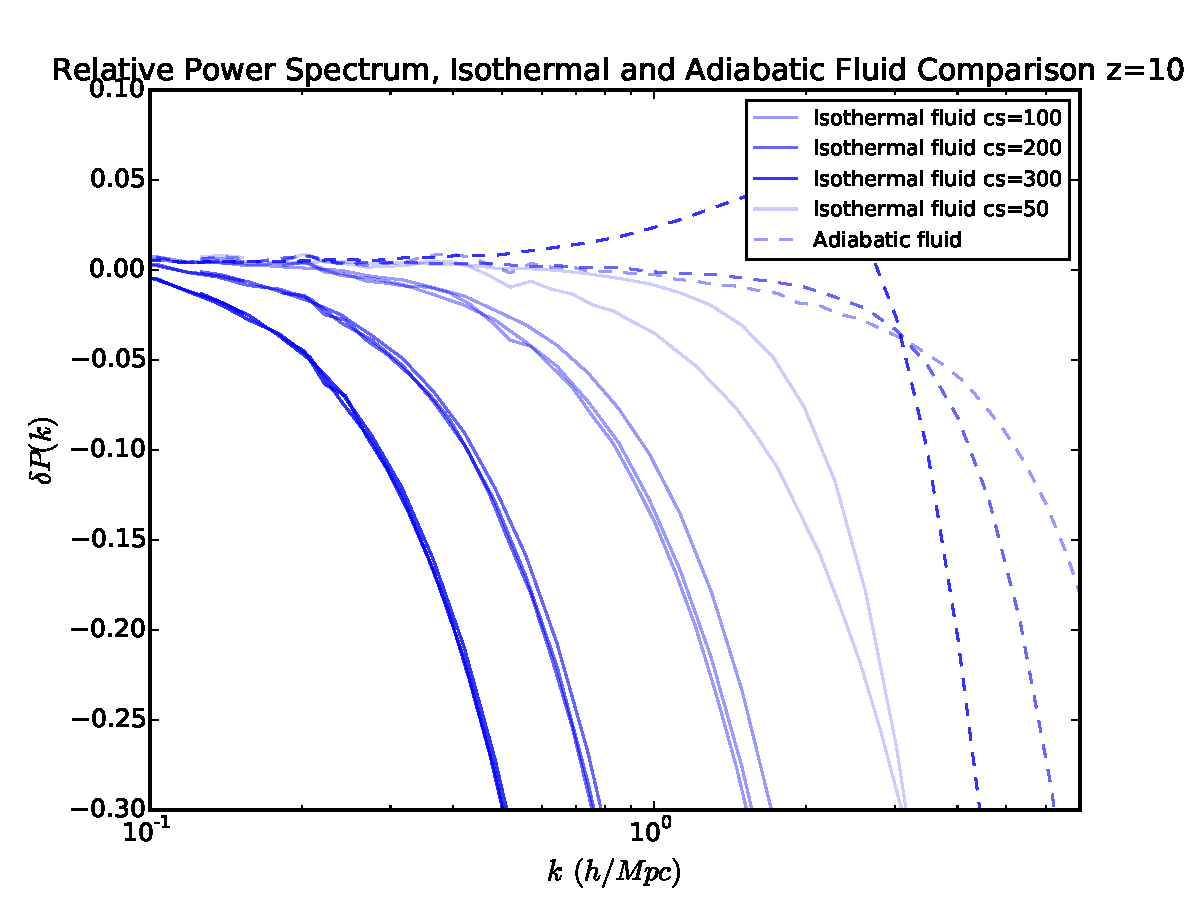
\includegraphics[width=0.48\textwidth]{z10fig}
\end{center}
\caption
{
}
\label{z10fig}
\end{figure}


\bibliographystyle{prsty}
\bibliography{references}

\end{document}

